\documentclass[12pt,a4paper]{article}

% Compatibilité avec les icônes éventuellement utilisées dans boites.sty
\usepackage{fontawesome5}
\providecommand{\faPencilAlt}{\faIcon{pencil-alt}}

\usepackage{styles/couleurs}
\usepackage{styles/mise_en_page}
\usepackage{styles/boites}
\usepackage{styles/maths}
\usepackage{styles/figures}

\usepackage{enumitem}
\usepackage{array}
\usepackage{tabularx}
\usepackage{amsmath}
\usepackage{amssymb}

\setlist[itemize]{
  leftmargin=1.5em,
  itemsep=0.18em,
  topsep=0.25em
}

\setlist[enumerate]{
  leftmargin=*,
  itemsep=0.22em,
  topsep=0.3em
}

\begin{document}

\begin{center}
  {\sffamily\LARGE\bfseries\color{TitreC}
  Séquence 3 -- Nombres relatifs}\\[0.2em]

  {\sffamily\large\bfseries\color{SavoirC}
  Produits, quotients et enchaînements de calculs}
\end{center}

%==================================================
\section{Multiplier deux nombres relatifs}
%==================================================

\subsection{Déterminer le signe du produit}

\propriete{Le produit de deux nombres relatifs :

\begin{itemize}
  \item de \textbf{même signe} est \textbf{positif} ;
  \item de \textbf{signes différents} est \textbf{négatif}.
\end{itemize}}

\begin{center}
\renewcommand{\arraystretch}{1.45}
\begin{tabularx}{0.82\textwidth}{
|>{\centering\arraybackslash}X
|>{\centering\arraybackslash}X|}
\hline
\textbf{Signes des facteurs}
&
\textbf{Signe du produit}
\\
\hline
\((+)\times(+)\)
&
\((+)\)
\\
\hline
\((- )\times(- )\)
&
\((+)\)
\\
\hline
\((+)\times(- )\)
&
\((- )\)
\\
\hline
\((- )\times(+)\)
&
\((- )\)
\\
\hline
\end{tabularx}
\end{center}

\subsection{Calculer un produit}

\exemple{
\[
(-3)\times(+7)
\]

Les deux facteurs ont des signes différents : le produit est négatif.

\[
3\times7=21
\]

Donc :

\[
(-3)\times(+7)=-21.
\]

De même :

\[
(-2{,}5)\times(-4)=+10.
\]}

\erreur{Il ne faut pas mélanger les règle des signes.

Par exemple :

\[
(-6)\times(-5)=+30
\]

et non \(-30\), car les deux facteurs ont le même signe.}

%==================================================
\section{Multiplier plusieurs nombres relatifs}
%==================================================

\subsection{Déterminer le signe}

\propriete{Dans un produit comportant plusieurs facteurs :

\begin{itemize}
  \item le produit est \textbf{positif} si le nombre de facteurs négatifs est \textbf{pair} ;
  \item le produit est \textbf{négatif} si le nombre de facteurs négatifs est \textbf{impair} ;
  \item le produit est \textbf{nul} si l'un des facteurs est nul.
\end{itemize}}

\exemple{
\[
A=(-2)\times3\times(-5)\times4
\]

Il y a deux facteurs négatifs. Comme \(2\) est pair, le produit est positif.

\[
A=2\times3\times5\times4=120.
\]

Donc :

\[
A=+120.
\]

Pour :

\[
B=(-2)\times(-3)\times(-4),
\]

il y a trois facteurs négatifs. Comme \(3\) est impair, le produit est négatif :

\[
B=-24.
\]}

\exemple{
\[
(-8)\times0\times(-21)=0.
\]

La présence d'un facteur nul suffit pour conclure.}
\newpage
%==================================================
\section{Diviser deux nombres relatifs}
%==================================================

\subsection{Le quotient comme facteur manquant}

\exemple{Pour calculer :

\[
(-42)\div(+6),
\]

on cherche le nombre qui vérifie :

\[
(+6)\times\ldots=-42.
\]

Comme :

\[
(+6)\times(-7)=-42,
\]

on obtient :

\[
(-42)\div(+6)=-7.
\]}

\subsection{Règle des signes}

\propriete{Le quotient de deux nombres relatifs :

\begin{itemize}
  \item de \textbf{même signe} est \textbf{positif} ;
  \item de \textbf{signes différents} est \textbf{négatif}.
\end{itemize}}

\begin{center}
\renewcommand{\arraystretch}{1.45}
\begin{tabularx}{0.82\textwidth}{
|>{\centering\arraybackslash}X
|>{\centering\arraybackslash}X|}
\hline
\textbf{Signes du dividende et du diviseur}
&
\textbf{Signe du quotient}
\\
\hline
\((+)\div(+)\)
&
\((+)\)
\\
\hline
\((- )\div(- )\)
&
\((+)\)
\\
\hline
\((+)\div(- )\)
&
\((- )\)
\\
\hline
\((- )\div(+)\)
&
\((- )\)
\\
\hline
\end{tabularx}
\end{center}

\exemple{
\[
(-35)\div(-5)=+7
\]

car les deux nombres ont le même signe.

\[
7{,}2\div(-4)=-1{,}8
\]

car les deux nombres ont des signes différents.}

\remarque{On ne peut jamais diviser par zéro.}

\erreur{Dans une division, on ne compte pas les signes comme dans un produit de plusieurs facteurs.
On compare seulement le signe du dividende et celui du diviseur.}

%==================================================
\section{Effectuer des enchaînements de calculs}
%==================================================

\subsection{Priorités opératoires}

\propriete{Dans une expression numérique :

\begin{enumerate}[label=\textbf{\arabic*.}]
  \item on commence par les calculs placés entre parenthèses ;
  \item on effectue ensuite les multiplications et les divisions, de gauche à droite ;
  \item on effectue enfin les additions et les soustractions, de gauche à droite.
\end{enumerate}}

\methode{Pour rédiger correctement un enchaînement :

\begin{itemize}
  \item effectuer une seule étape à la fois ;
  \item recopier sans les modifier les parties qui ne sont pas encore calculées ;
  \item écrire une nouvelle ligne après chaque transformation ;
  \item conserver les parenthèses autour des nombres négatifs tant qu'elles sont utiles.
\end{itemize}}

\exemple{
\[
A=(-24)\div(-6)+5\times(-2)
\]

On effectue d'abord la division et la multiplication :

\[
\begin{aligned}
A&=4+(-10)\\
 &=-6.
\end{aligned}
\]}

\exemple{
\[
B=\bigl(8-3\times(-2)\bigr)\div(-7)
\]

\[
\begin{aligned}
B
&=\bigl(8-(-6)\bigr)\div(-7)\\
&=14\div(-7)\\
&=-2.
\end{aligned}
\]}

\exemple{
\[
C=(-3)\times(4-7)-18\div(-6)
\]

\[
\begin{aligned}
C
&=(-3)\times(-3)-(-3)\\
&=9-(-3)\\
&=12.
\end{aligned}
\]}

\erreur{On ne regroupe pas une addition avec une multiplication sans parenthèses.

Par exemple :

\[
18-(-3)\times4
\]

ne devient pas :

\[
(18-(-3))\times4.
\]

Le calcul correct est :

\[
18-(-3)\times4
=
18-(-12)
=
30.
\]}

\subsection{Multiplications et divisions successives}

\remarque{La multiplication et la division ont la même priorité.
On les effectue donc de gauche à droite.}

\exemple{
\[
24\div(-6)\times(-2)
\]

\[
\begin{aligned}
24\div(-6)\times(-2)
&=(-4)\times(-2)\\
&=8.
\end{aligned}
\]}

\erreur{
\[
24\div(-6)\times(-2)
\neq
24\div\bigl((-6)\times(-2)\bigr).
\]}

%==================================================
\section*{Synthèse}
%==================================================

\aretenir{
\begin{itemize}
  \item Pour un produit ou un quotient de deux relatifs :
        même signe \(\Rightarrow\) résultat positif ;
        signes différents \(\Rightarrow\) résultat négatif.
  \item Pour un produit de plusieurs facteurs :
        un nombre pair de facteurs négatifs donne un produit positif ;
        un nombre impair donne un produit négatif.
  \item Un produit comportant un facteur nul vaut \(0\).
  \item Dans un enchaînement, on respecte les parenthèses puis les priorités opératoires.
  \item Avant d'utiliser la calculatrice, on prévoit le signe et un ordre de grandeur.
\end{itemize}}

\vspace{0.5cm}

%==================================================
\section*{Synthèse -- Carte mentale}
%==================================================

\vspace{1cm}

\begin{center}
    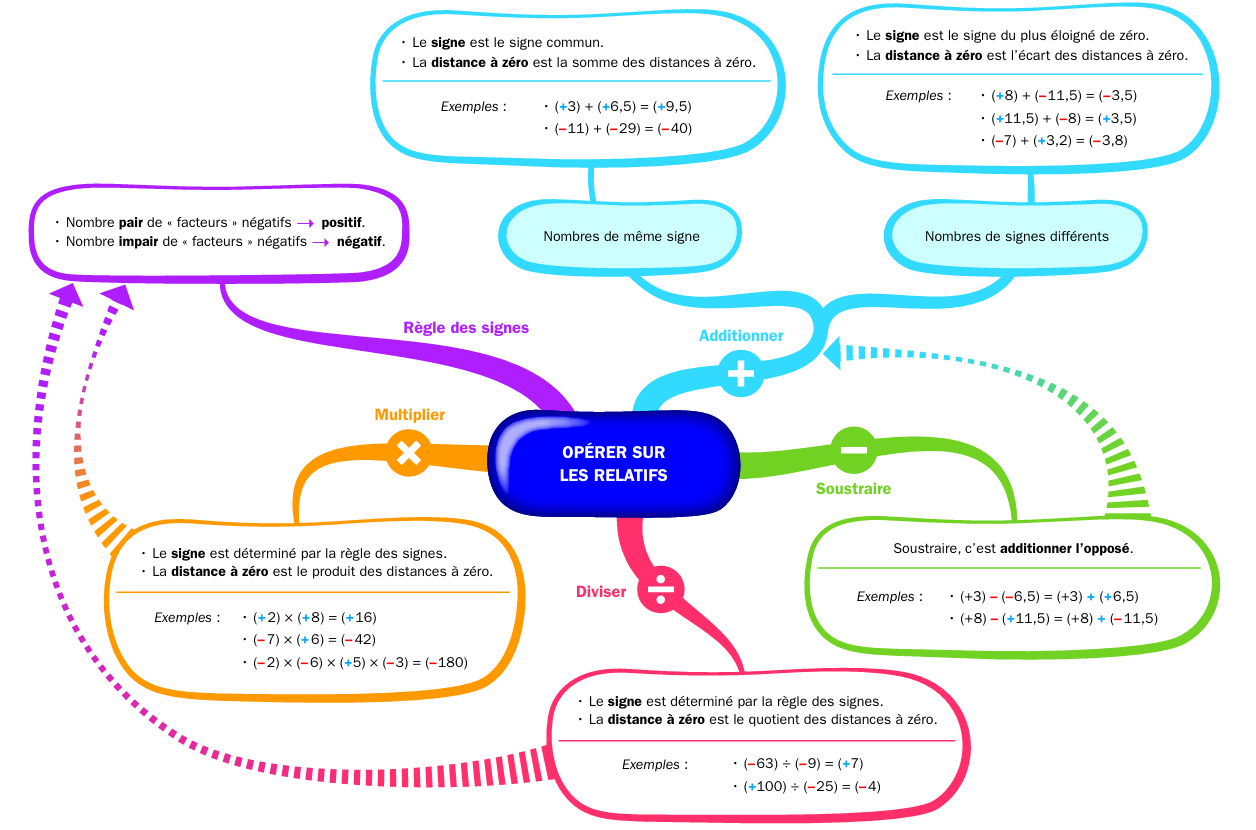
\includegraphics[width=1\linewidth]{images/cm_relatifs.png}
\end{center}

\end{document}
